\documentclass[11pt, oneside]{article}   	% use "amsart" instead of "article" for AMSLaTeX format
\usepackage{geometry}                		% See geometry.pdf to learn the layout options. There are lots.
\geometry{letterpaper}                   		% ... or a4paper or a5paper or ... 
%\geometry{landscape}                		% Activate for for rotated page geometry
%\usepackage[parfill]{parskip}    		% Activate to begin paragraphs with an empty line rather than an indent
\usepackage{graphicx}				% Use pdf, png, jpg, or eps§ with pdflatex; use eps in DVI mode
								% TeX will automatically convert eps --> pdf in pdflatex		
\usepackage{amssymb}
\usepackage{amsmath}
\usepackage{parskip}
\usepackage{color}
\usepackage{hyperref}

\title{Quadratic}
%\author{The Author}
%\section{}
%\subsection*{}
\date{}							% Activate to display a given date or no date

\graphicspath{{/Users/telliott_admin/Dropbox/Tex/png/}}
% \begin{center} 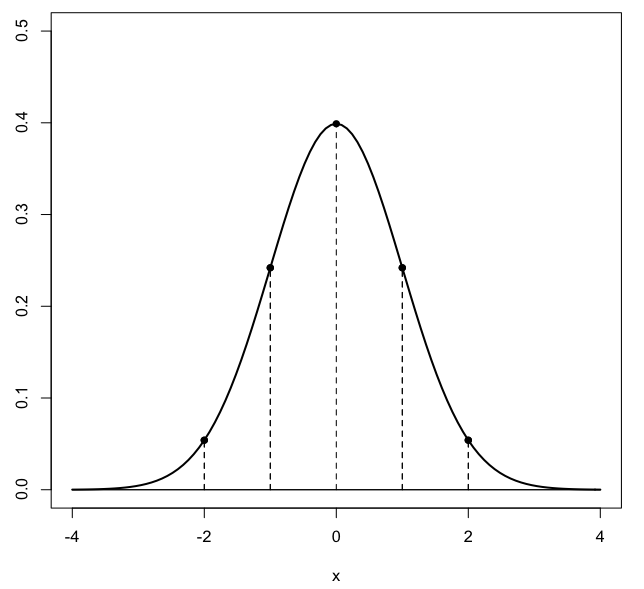
\includegraphics [scale=0.4] {gauss3.png} \end{center}
\begin{document}
\maketitle
\Large
We want to solve
\[ y = ax^2 + bx + c \]
We suppose that $a \ne 0$ (since this is a quadratic, after all), so we can divide by $a$ on both sides:
\[ \frac{y}{a} = x^2 + \frac{b}{a} x + \frac{c}{a} \]
Rearranging a bit 
\[ \frac{y}{a} -  \frac{c}{a} = x^2 + \frac{b}{a} x \]
Our particular interest is in the value(s) for $x$ when $y=0$ so that leaves:
\[ -  \frac{c}{a} = x^2 + \frac{b}{a} x \]
The crucial insight is to see that the right-hand side is nearly a perfect square
\[ x^2 + \frac{b}{a} x + ?? \]
similar to 
\[ (x + m)^2 = x^2 + x(2m) + m^2 \]
The coefficient of $x$ on the right-hand side is $2m$.  

In our problem we have $b/a$ so we decide to try $2m = b/a$, which works
\[ (x + \frac{b}{2a})^2 = x^2 + \frac{b}{a} x + \frac{b^2}{4a^2} \]

Now that we know what to do, go back to the original equation
\[ -  \frac{c}{a} = x^2 + \frac{b}{a} x \]
add the same term (what we called $m^2$) to both sides
\[ -  \frac{c}{a} + \frac{b^2}{4a^2} = x^2 + \frac{b}{a} x + \frac{b^2}{4a^2} \]
write our perfect square
\[ -  \frac{c}{a} + \frac{b^2}{4a^2} = (x + \frac{b}{2a})^2 \]

Almost there.  Multiply both sides by $4a^2$
\[ -  4ac + b^2 = 4a^2(x + \frac{b}{2a})^2 \]
That should look familiar.  

Switch the order of terms on the left and take (both negative and positive) square roots:
\[ \sqrt{b^2 - 4ac} = \pm \ 2a(x + \frac{b}{2a}) \]
\[ \pm \ \sqrt{b^2 - 4ac} = 2a(x + \frac{b}{2a}) \]
\[ - \frac{b}{2a} \pm \ \frac{\sqrt{b^2 - 4ac}}{2a} = x \]
\[ x = \frac{-b \pm \ \sqrt{b^2 - 4ac}}{2a} \]

\subsection*{version 2}

Another approach that I've seen which is counterintuitive (at least to start with).  Start by saying explicitly we want the zeroes:

\[ ax^2 + bx + c = 0 \]
\[ x^2 + \frac{b}{a} x = -\frac{c}{a} \]
Make the inspired substitution:
\[ x = t - \frac{b}{2a} \]
Then
\[ x^2 = t^2 - \frac{b}{a}t + \frac{b^2}{4a^2} \]
\[ \frac{b}{a}x = \frac{b}{a}t - \frac{b^2}{2a^2} \]
So we have then:
\[  t^2 - \frac{b}{a}t + \frac{b^2}{4a^2} +\frac{b}{a}t - \frac{b^2}{2a^2} = -\frac{c}{a} \]
One set of cancellations
\[  t^2 + \frac{b^2}{4a^2} - \frac{b^2}{2a^2} = -\frac{c}{a} \]
and another, with rearrangement
\[  t^2 = -\frac{c}{a} + \frac{b^2}{4a^2} \]
Place over a common denominator and take the square roots
\[ t^2 = \frac{4ac - b^2}{4a^2} \]
\[ t = \pm \frac{\sqrt{b^2 - 4ac}}{2a} \]
Reverse the substitution:
\[ x = \pm \frac{\sqrt{b^2 - 4ac}}{2a} - \frac{b}{2a} \]
Finally
\[ x = \frac{- b \pm \ \sqrt{b^2 - 4ac}}{2a} \]

\subsection*{version 3}
Here is a third approach.  We wish to find the values of $x$ that make this statement true:
\[ ax^2 + bx + c = 0 \]
\[ x^2 + \frac{b}{a} x + \frac{c}{a} = 0 \]
Suppose that $x = m$ and $x = n$ are the two solutions.  That means:
\[ x^2 + \frac{b}{a} x + \frac{c}{a} = (x - m)(x-n) \]

Now, expand the right-hand side
\[ x^2 + \frac{b}{a} x + \frac{c}{a} = x^2 - (m + n)x + mn \]
it is clear that the coefficients of $x$ on each side must be equal to each other:
\[ -(m+n) = \frac{b}{a} \]
\[ m+n = -\frac{b}{a} \]

Next we work on the constant term $mn$.  A little algebra gives:
\[ (m+n)^2 = m^2 + 2mn + n^2 \]
\[ (m-n)^2 = m^2 - 2mn + n^2 \]
Subtract
\[ (m+n)^2 - (m-n)^2 = 4mn \]
\[ mn = (m+n)^2 - (m-n)^2 - 3 mn \]

Going back to what we had above
\[ x^2 + \frac{b}{a} x + \frac{c}{a} = x^2 - (m + n)x + mn \]
We see that
\[ \frac{c}{a} =  mn = (m+n)^2 - (m-n)^2 - 3 mn \]
So
\[ (m - n)^2 = \frac{c}{a} - (m+n)^2 + 3mn \]
But $c/a = mn$ so
\[ (m - n)^2 = 4\frac{c}{a} - (m+n)^2 \]
Recall that $m+n = -b/a$
\[ (m - n)^2 = 4\frac{c}{a} - (\frac{b}{a})^2 \]
\[ m - n = \sqrt{4\frac{c}{a} - (\frac{b}{a})^2} \]
Together with what we found above
\[ m + n = -\frac{b}{a} \]
When solved simultaneously, these two equations give the result we seek.  Addition gives
\[ 2m = \sqrt{4\frac{c}{a} - (\frac{b}{a})^2} -\frac{b}{a} \]
Subtraction gives
\[ 2n = -\frac{b}{a} - \sqrt{4\frac{c}{a} - (\frac{b}{a})^2} \]
which has just flipped the sign on the square root term.  Thus $m$ and $n$ differ only in the sign of that term.

Let's clean up the result
\[ 2m = \sqrt{\frac{4ac}{a^2} - (\frac{b}{a})^2} -\frac{b}{a} \]
Factor out the $\sqrt{1/a^2}$
\[ 2m = \frac{\sqrt{4ac - b^2}}{a} -\frac{b}{a} \]
\[ m = \frac{-b + \sqrt{4ac - b^2}}{2a} \]



\end{document}